\section{Introduction}
\label{sec::intro}
%
In an era where most user activity is electronically recorded, the data analysts can gain insights into user behavior by mining the large amounts of accumulated data.
\emph{Cohort analysis}, originating from social science\cite{glenn2005cohort}, fits well into the analysis of user behavior by collectively exploring the impact of two factors, namely \emph{social change} and \emph{age}, which are considered to be the major source affecting user behavior. Typically, cohort analysis groups users into different cohorts based on how they perform certain activities of interest, and measures how the behavior of each cohort evolves with time thereafter. Below is a real-world application of cohort analysis in healthcare.
%With the maturity of data storage and cleansing techniques, we are increasingly keen on analyzing and explaining the data from new angles instead of optimizing the old-fashioned data analysis methods.

\emph{\textbf{Example:} A hospital wants to know the side effects of a new medicine A on patients cohorted by different physical ages who are diagnosed with disease B. The patient is monitored after taking the medicine at least 2 times by observing abnormal values in daily-conducted lab-test C.}


However, cohort analysis brings in two new challenges that standard analytic techniques, such as SQL Query, cannot easily overcome. First, it is difficult and time consuming to compose correct SQL queries for cohort analysis, especially for those without a strong database background. Second, due to the complex GROUP BY and JOIN operators involved in the query, the efficiency of leveraging traditional database for cohort analysis is extremely low~\cite{jiang2016cohort}. %, especially for those analysis in new angles. 
%Specifically, cohort analysis needs to collect users who change their behaviors over time dimension.
%To implement this, plentiful complicated GROUP BY and JOIN operators are needed, which undoubtedly consumes quite a long time to process.
% For instance, we need plentiful complicated GROUP BY and JOIN operators to select the users who change their behaviors over time.

COHANA~\cite{jiang2016cohort} was recently proposed to tackle the efficiency (i.e., the second) challenge.
This work encompasses the design of cohort operators and implements an efficient cohort query processing engine. It defines cohort query in a more concise and accurate standard than its SQL equivalent, and the specially designed storage manager and query executor in COHANA grants performance superiority against traditional database systems. 

However, the complexity of building the cohort query, which is another challenge for data analysts using traditional SQL tools, is still unaddressed by COHANA according to our experience of industrial deployment, in collaboration with multiple organizations. The major complexity lies in the various terms and options that are involved in the queries submitted to COHANA, but difficult to understand for industrial clients.
%The following example is a practical scenario for cohort analysis in medical fields:


%There are two decisive factors affecting user behavior in cohort analysis: age and social change. Here, age is defined by the number of passed time unit after the selected user fulfill certain given behaviour patterns while social change is how the entire society evolves over the time. 
%Cohort analysis studies user behavior by introducing the concept of \textbf{birth event}, which determines the birth time and identifies the \textbf{cohort} for each user according to the given cohort composition. Then, the \textbf{age} of each user activity is derived from the time passed since the first birth event. Finally, an \textbf{aggregation} method is used to measure how the behavior of users in each cohort evolves over age.
% The following example is a practical scenario for cohort analysis in medical fields.


%To solve the problem described in the example, complex GROUP BY and JOIN operators must be imported in traditional databases with precise order and expressions.
%Medicians may spend hours to write such a query even with adequate computer science background, no matter how long is going to cost for the database to process.
% Furthermore, it is painful to compose the correct SQL queries for the example.
%Moreover, although COHANA engine can efficiently handle this example, it is still hard to understand the terms used in the query submitted to the engine for the medicians.
%Thus. they are often unable to compose the correct query format.

% To solve the problem described in the example, complex GROUP BY and JOIN operators must be imported in traditional databases.
% Furthermore, it is painful to compose the correct SQL queries for the example.
% Nonetheless, this example can be readily mapped onto a cohort analysis task, as we shall see below.
%cohort analysis can be easily mapped   handle this example with the aforementioned definitions.
% Though it is troublesome to solve for SQL GROUP BY, the problem can be handled easily by cohort analysis by determining the three definitions are well defined.


% Despite all the efforts done in COHANA system, we find out that it is still cumbersome to build cohort queries as easy as we expect.
To overcome this issue, we propose a web tool that runs on top of COHANA to provide users with an intuitive and practical cohort querying service. 
This tool lets users determine the parameters of cohort analysis by selecting options described in natural language on the web page, instead of writing queries accepted by COHANA, which are of a json format.  
It is especially helpful for analysts who lack the knowledge of defining the cohort analysis in pre-defined terminologies.%, such as ``age" and ``birth event". 
Furthermore, the result of the cohort query returned by COHANA is visualized,
which plays a key role for the analysts to evaluate their queries and generate business reports.
Generally, the ultimate goal of this tool is to help analysts gain insights to the data swiftly, accurately, and intuitively.

In this demo paper, we will give an overview of our system by introducing key concepts in cohort analysis along with our system architecture first. We then demonstrate the entire analysis process in the context of the running example, including the data preparation, cohort selection, and result visualization.
Although our demo is a general tool for cohort analysis, we shall focus on the medical area in the rest of this paper for better illustration and explanation.

\section{System Overview}
In this section, we start with three key definitions presented in all cohort queries, and then depict the overall system architecture.  

\subsection{Query Definition}
In cohort analysis, the behavior user performed are called ``event", which is usually recorded as a string column in database. 
There are four key concepts presented in the COHANA paper~\cite{jiang2016cohort}, i.e., \textbf{User Birth}, \textbf{Cohort}, \textbf{Age} and \textbf{Metric}.
However, to define the cohort query in a more powerful way, the definitions are further extended as following:
% A typical cohort analysis requires the definition of \textbf{birth},  \textbf{age}, \textbf{metric} and \textbf{cohort}. 

\textbf{User Birth}: A user is selected into the cohort query result if and only if the user performs a given sequence of events. This selection is called ``user birth" and the given sequence is called ``birth events" accordingly. It is worth noting that a event sequence, instead of a single event, is employed to make the selection more precise and comprehensive.
For the running example, the birth events are defined as taking medicine A twice.
%the patient has taken medicine A at least twice; (2) the patient is observed abnormal values in lab-test C afterwards.

\textbf{Cohort}: Cohort refers to a group of users sharing certain common characteristics when born. In other words, a user is born immediately after completing the birth events and enters a cohort accordingly. For the running example, the patients who perform the birth events are cohorted by one of their common characteristics, namely the physical age.
%It is worth noting that although a user's characteristics may change over time, its cohort is determined by the characteristics that user has at the time of birth.

\textbf{Age}: The age of a selected user is defined as the number of time units passed since its birth. Two types of time units are supported in the query. The first one is calendar time unit, such as day/week/month. For example, if we define the birth event as taking lab test and the time unit as one day, a patient whose first recorded lab test is on January 1st will be at age 1 on January 2nd. 
Another patient taking the same lab test on March 4th for the first time will also be at age 1 on March 5th, regardless of the difference in birth times. The other age type is defined by the occurrence of a certain event. For example, we can use the admission to define the age of patients such that a patient is at age 1 before the first admission since born.
The patient will be at age 2 if unfortunately he is sick again and get re-admitted by the hospital.


\textbf{Metric}: Metric refers to the result of user-defined calculation function, denoted as metric function and performed on the generated cohorts within a same age. Users can define metric function as simple aggregations like counting the number of occurrences of a particular event, or as complicated validation like fitting a probability distribution. For example, we can check the retention rate of patients' re-admission to the hospital by counting patients' admission records every month (i.e., one unit of age) after being discharged at the first time (i.e., the birth event).

%Cohort analysis fits well into the analysis of user behavior by collectively exploring the impact of two factors, namely \emph{social change} and \emph{age}, which are considered to be the major source affecting user behavior. Typically, for a set of selected users, cohort analysis groups them into different cohorts based on how they perform a certain birth event, and measures how the behavior of each cohort evolves with time thereafter.

\subsection{System Architecture}

\begin{figure}
    \centering
    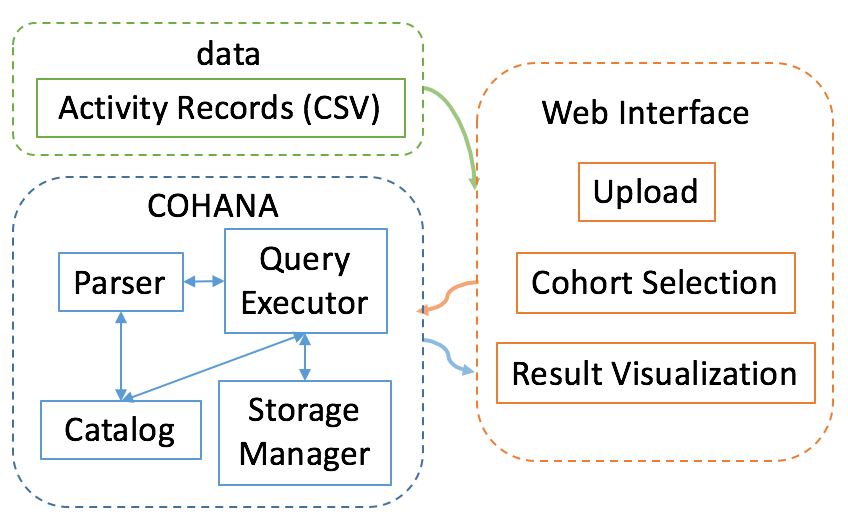
\includegraphics[width=0.4\textwidth]{arch.png}
    \caption{System Architecture}
    \label{fig:sys_arch}
\end{figure}

Figure \ref{fig:sys_arch} outlines the system architecture of the entire system. The input of the system is the data in the green rectangle and there are two components of the system, i.e., the COHANA engine and the web interface, which are respectively surrounded by a blue and orange rectangle. 

The input of the system is actually a file containing the all the user records in the CSV format. 
Besides user behaviors and the associated timestamp, the file can also 
%The only data we required is a CSV file of user activity records, 
including user details and other information.
The data records of a single user are cluster together in chronological order. 
This sorting alignment for the records is a ubiquitous format for data analysis, and it aids the COHANA engine in the detection of the tuples containing users' birth activities.

The COHANA engine consists of a parser, a catalog, a query executor and a storage manager, wherein the last two components are the cores to support efficient cohort analysis queries. 
Compared to the original system presented in ~\cite{jiang2016cohort}, new functionalities are added to further make the query result much more readable and traceable.
For example, the user can name the cohort, or the set of cohorts, generated by the query, for further usage.
This is helpful for doctors to find the effective target for a new medicine. 
A practical use case can be: the doctor first discovers the patients for which a medicine of interest is effective,
and then groups those patients into difference cohorts based on their diseases. Then, the doctor can look into one specific disease and further profile the patients in this disease cohort by their ages, genders, diagnosing histories, etc.
% such as the birth-user selection, which is  of qualified users, the age selection operator to retrieve activity tuples satisfying certain conditions, and the cohort aggregation operator to apply certain metrics on tuples.

The storage manager applies a chunking scheme and a series of compression techniques. Specifically, it partitions the data horizontally as chunks such that each chunk has approximately the same number of activity records and all activity records of a single user are included in a single chunk. Afterwards, different compression schemes are employed on each column depending on the data type of this column, e.g., Run-Length-Encoding technique is used for user identity column while two-level compression is used for string columns ~\cite{jiang2016cohort}. %For columns containing integers, delta encoding scheme is employed. 

The query executor generates a logical query plan using an operator tree from the original cohort query and optimizes the plan by pushing the birth selection (i.e., find users who fulfill the birth sequence and allocate them into respective cohorts) into the bottom level of the tree. After scanning each data chunk in the storage manager, the query executor merges and presents the results of the submitted query.

The query processing in COHANA is extremely fast compared to traditional approaches in SQL due to the customized storage layout in storage manager and optimized cohort operators. As reported in~\cite{jiang2016cohort}, it is 10x and 100x faster than SQL solutions in MonetDb\cite{boncz2005monetdb} and Postgresql\cite{momjian2001postgresql}, respectively.

The interactive web interface for COHANA is implemented under Django\cite{django} framework with Gentelella\cite{gentelella} template. We also employ ECharts 2.0\cite{echarts}, a charting library, to support massive chart manipulations in our system. 
The web interface is responsible for all front-end user interactions such as uploading the dataset, constructing queries, and visualizing results. 
It is also in charge of back-end data transfer and interactions with COHANA engine. 

When applying the cohort analysis for their own dataset, users first import the dataset to be analyzed into COHANA engine via the user interface by either uploading the raw data or specifying a web address.
The back end receives the dataset and pass the dataset to the engine, extracting the needed column information for compression in a cohort analysis page. 
Then, users map their analysis task from natural language to cohort query definitions, including the user selection, cohort definition, age specification and metric calculation.
This mapping is done easily with simple and clear options provided in the front end as we shall see below.
Next, the options selected are translated into the format accepted by COHANA engine on the back end, which is further passed to the engine. 
Finally, the processed result is sent back from COHANA engine and parsed by the back end. The front end visualizes the parsed result into tables or charts for users reference.

\section{Demonstration Outlines}

In this section, we elaborate on the data preparation, the query selection, and result visualization with the aforementioned medical example in Section~\ref{sec::intro} to explain cohort analysis process using our system. This example is quite representative in the medical context according to the doctors in collaboration.
Although the data we use for this demonstration is not real due to confidential issues, we indeed force the fake dataset to follow the schema of the real health care records and the distribution of the original dataset.
It is worth mentioning that while the example resides in the medical domain, such analysis is common in various other domains and can likewise be elegantly handled by our system.

\subsection{Data Preparation}

Overall, we have eight columns in the CSV dataset, i.e., \emph{id, birthyear, event, disease, medicine, labtest, value, and time}. \emph{id} is a unique identifier for each patient, and \emph{birthyear} and \emph{time} are unambiguous. 
\emph{Event} contains the real affairs the user experiences.
There are three options, ``diagnose", ``prescribe" and ``labtest" in the \emph{event} column.
The \emph{disease} column contains a particular code for the illness diagnosed when a patient is admitted if the \emph{event} is ``diagnose", otherwise it is a default value set by the user.
%A fact in the reality here is that even though a patient can be in the hospital for more than one day, he or she might have only one recorded diagnosis for the entire visit. 
The \emph{medicine} column indicates the prescription issued to the patient. %and may not cover all the days of his hospitalization. 
The \emph{labtest} refers to the type of tests patients take and the \emph{value} presents integral test result. 

An example in the dataset is shown in Figure \ref{fig:upload}. The patient with id P-0 was admitted to the hospital on 1st January 2012, diagnosed with Disease-B, prescribed Medicine-C, and scored 44 on Labtest-C. On the next day, he scored 25 on the same lab test. 
It is worth noting that there exist redundancies in the records, which is common for real medical scenarios. 
The storage manager in the COHANA engine will compress the data intelligently to assure low storage consumption and high query efficiency.
%, provided the User ID, event and time columns are sorted in the manner as described in the previous section.

% \end{figure}


\begin{figure*}
\begin{minipage}{0.3\textwidth}
% \begin{subfigure}{0.3\textwidth}
    \centering
    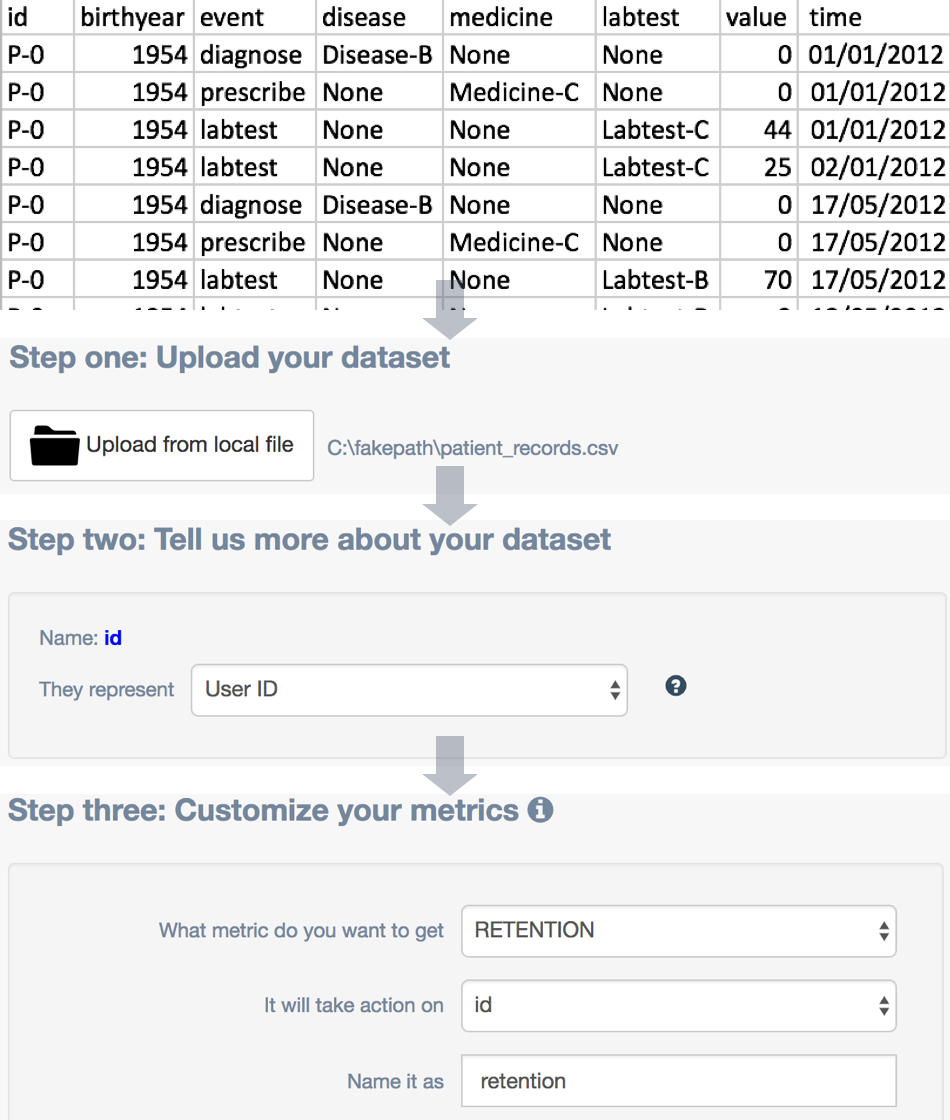
\includegraphics[width=0.9\linewidth]{upload_all_vertical.png}
    \caption{Data Upload}
    \label{fig:upload}
% \end{subfigure}%
\end{minipage}
\begin{minipage}{0.38\textwidth}
% \begin{subfigure}{0.4\textwidth}
    % \centering
    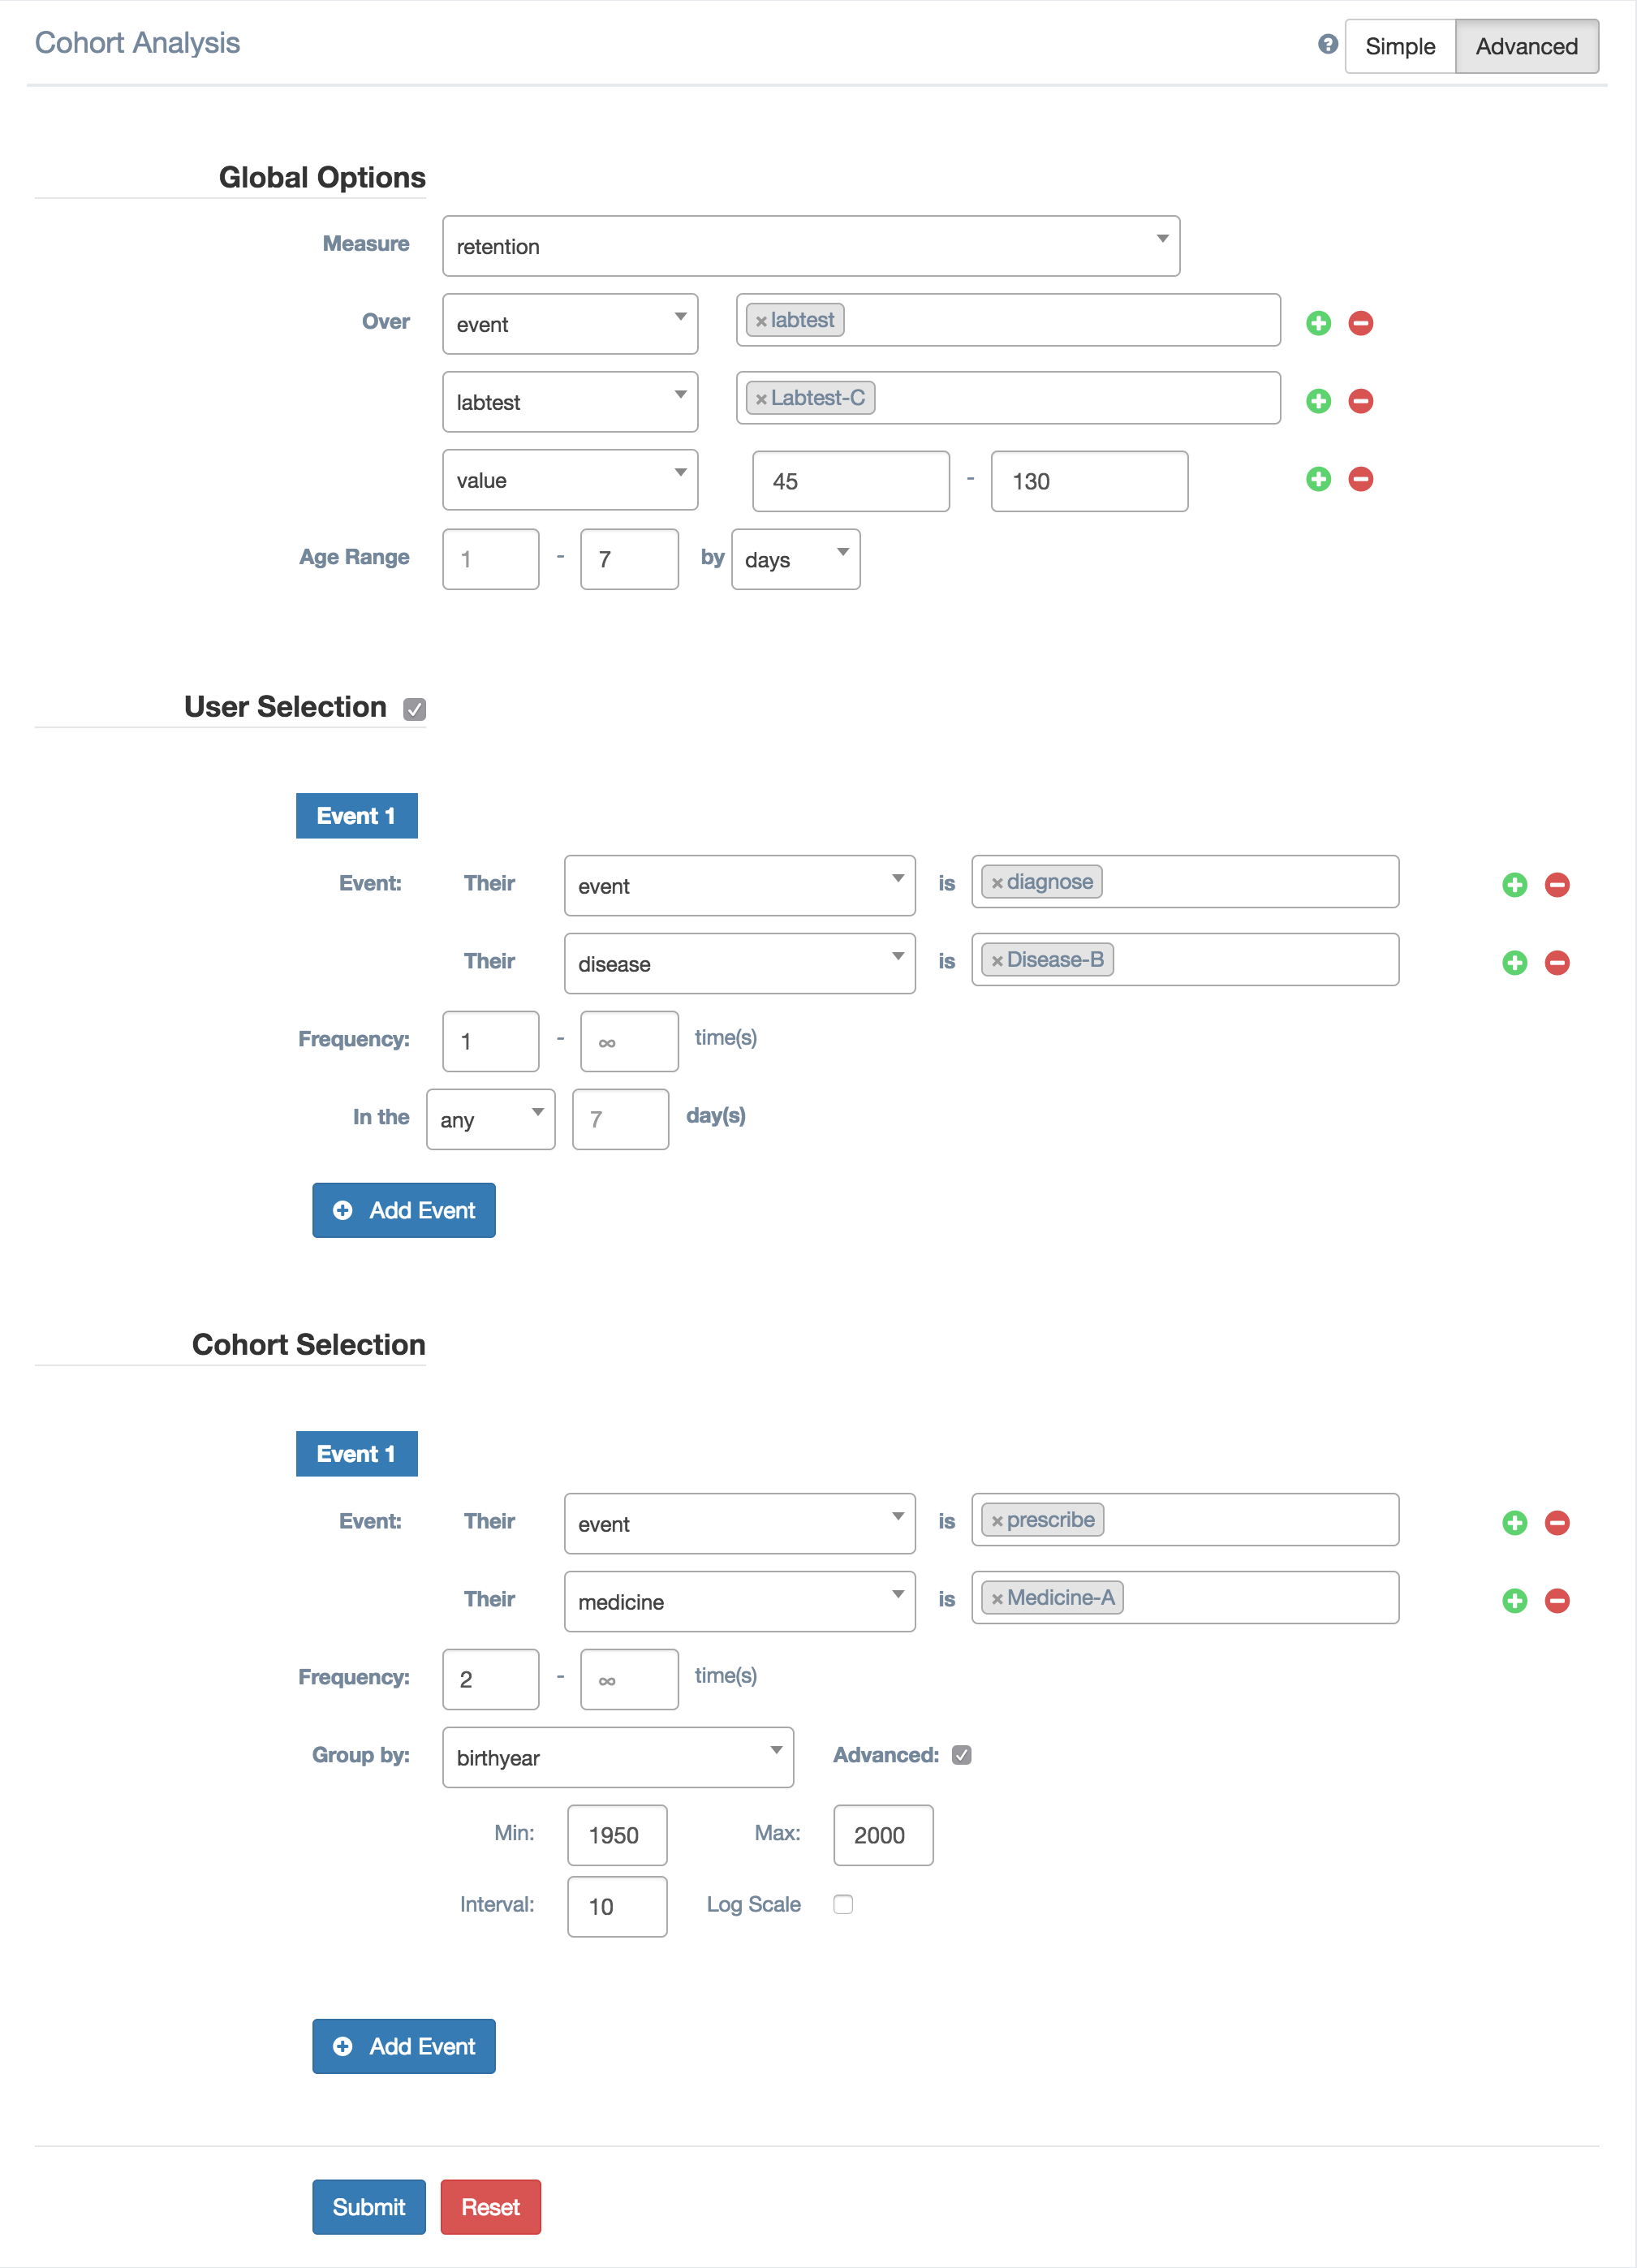
\includegraphics[width=0.96\linewidth]{query.png}
    \caption{Cohort Selection}
    \label{fig:cohort}
% \end{subfigure}%
\end{minipage}
\begin{minipage}{0.3\textwidth}
% \begin{subfigure}{0.3\textwidth}
    % \centering
    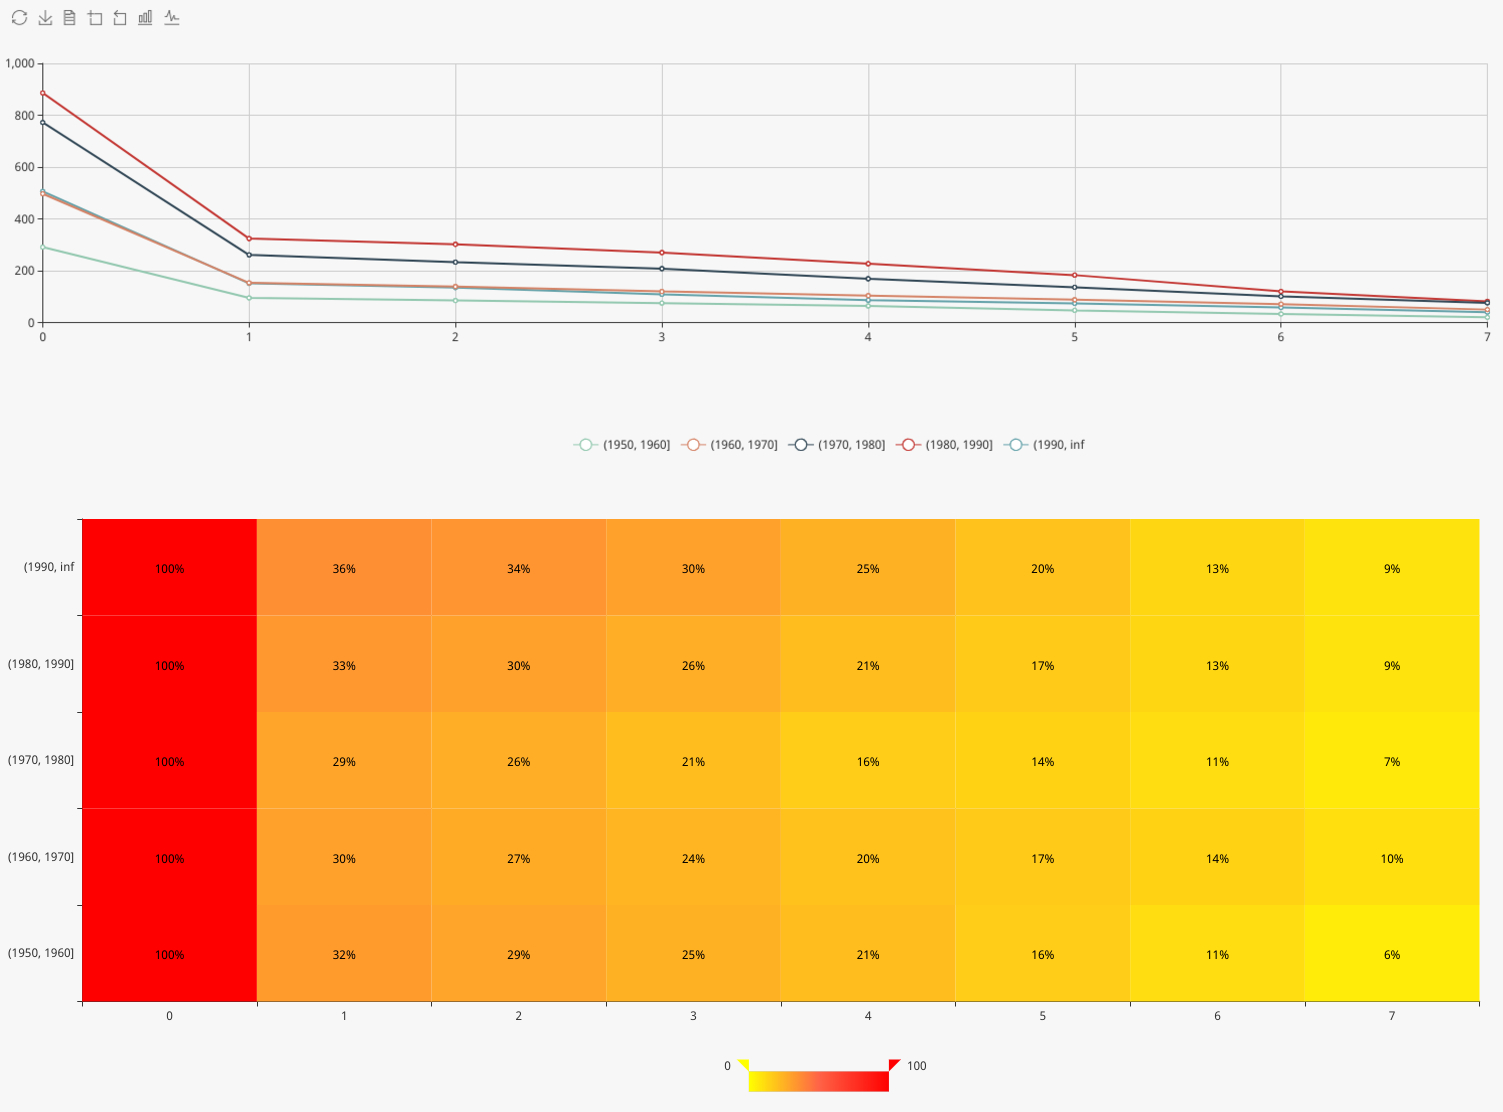
\includegraphics[height=20em, width=0.99\linewidth]{image.jpg}
    \caption{Result Visualization}
    \label{fig:visual}
% \end{subfigure}%
\end{minipage}

% \caption{Web Interface}
\end{figure*}

\begin{table}[tb!]
\begin{center}
    \begin{tabular}{ |c|c| }
        \hline
        Options & Description \\[0.5ex] 
        \hline\hline
        User ID & user identity \\
        \hline
        Event & action the user performs\\
        \hline
        Attributes & other string columns\\
        \hline
        Values & other integer columns\\
        \hline
        Time & action time \\
        \hline
    \end{tabular}
\end{center}
\caption{Schema Selection for the Dataset}
\label{table:schema}
\end{table}

\begin{table}[tb!]
\begin{center}
    \begin{tabular}{ | c | c | }
        \hline
        Options & Description \\[0.5ex] 
        \hline\hline
        RETENTION & number of users \\
        \hline
        COUNT & number of records \\
        \hline
        SUM & sum of certain integer column \\
        \hline
    \end{tabular}
\end{center}
\caption{Metrics Selection for the Dataset}
\label{table:metrics}
\end{table}

The first step we need to conduct cohort analysis is to upload the CSV file and specify the schema of the data and the metrics to be evaluated as shown in Figure \ref{fig:upload}. 
The descriptions for the options regarding the schema and metrics are shown in Table \ref{table:schema} and \ref{table:metrics}. 
Here, we choose RETENTION as our metric for this problem to reflect the number of qualified patients in each age since their birth. 
The web interface allows for assigning multiple metrics, such as choosing COUNT on the labtest column if the number of abnormal values is needed, or using SUM for the total occurrences of abnormal values. 
After COHANA engine receives the dataset and its specifications, the web application navigates the user to the cohort analysis page where options are equipped with the content found in the records.

\subsection{Cohort Selection}

According to the running example, a decomposition of the natural language can be formed: 1) only patients diagnosed with disease B are needed for the analysis; 2) the birth events for patients are taking medicine A twice; 3) the time unit of age is one day; and 4) the metrics are collected by counting patients that with abnormal values in lab-test C. 
Following the decomposition, the options provided on the web page can be chosen easily, as shown below.

As depicted in \ref{fig:cohort}, in the ``Cohort Metric" panel, we measure the \emph{retention} defined in last step over patients who experience ``labtest" event with type ``Labtest-C" and have a score between 45 to 130. 
The measured period, namely the range of the age, is from 1 to 7 days after users' birth.
The range of the age here defines the time period over which patients' behavior are measured. For instance, a small range can be chosen for short-term effects while a large range can be selected for long-term effect.

The next selection is on the group of user to include in our analysis as shown in ``User Selection" panel. This part can be omitted if the analysis is conducted over all users. 
In the figure, the patients who experience event ``diagnose" with diagnosing result ``Disease-B" within any week are specified as the target users.
More constraints on user selection can be cast by ticking the \textbf{+} button on the ``Event" line.
%For example, the valid range of user records can be indicated via the web interface.

For ``Birth Criteria" panel, the birth event ``prescribe" and the corresponding medicine ``Medicine-A" are specified as shown in the figure.
In addition, a patient should take the medicine at least twice before being 
born as the frequency of this birth event is at least 2.
If multiple birth events are assigned by ticking the \textbf{+} button, a 
patient is regarded to be born only when all the birth events are fulfilled. 
In the last part of this panel, the user indicates that the patients should be grouped further by their birthyear in the range of \emph{1950 to 2000} with a scale of 10 years.

\subsection{Result Visualization}

Within seconds of submitting the cohort selection, a line chart and a heat map of the cohort analysis result will be displayed as shown in Figure~\ref{fig:visual}. In the line chart, the x-axis represents the \emph{age} of the patients since their {birth} --- the number of days after taking Medicine A twice in our context --- and the y-axis represents the aggregation result, i.e., the number of patients with abnormal values detected by Labtest-C. The value of y-axis on {age 0} is the total number of patients {born} to the cohort. 
Each line stands for a cohort of patients as grouped by the decade they were born in. 
This line chart, answering the cohort query numerically, not only illustrates the trend of user behavior along the time axis, but also offers a view of
the difference in the behavior of different cohort patients.

The bottom heat map is axised with {age} and cohort group. 
A cell $(i,j)$ in the heat map represents the proportion of patients in cohort $i$ that are detected with an abnormal Labtest-C value at age $j$. 
%The first column, which represents {age 0}, will always have the value 100\%. 
Having cells be shaded with different color depths in accordance to its metric value gives spontaneous expression on the evolvement of patient behavior in terms of Labtest-C result, and also indicates deep insight into patient behavior between different cohorts. 

The two charts explain the result of the submitted cohort query in an absolute and relative manner respectively. We can observe from these two charts that younger patients are actively exhibiting side effects, suggested by the high values in group (1980, 1990] in the line chart, while elder patients take longer to get accustomed to the medicine.%, as elderly cohorts retain color for a longer time in the heatmap.

Additionally, with the help of ECharts\cite{echarts}, we provide a wide variety of operations to manipulate the chart, such as zooming in and changing the chart type, as shown in the toolbar above the chart. These functions afford immediate responses to visualization exploration which is helpful for further data excavation.

\section{Related Work and Conclusion}

Recently, due to the increasing volume of internet user behavioral data, cohort
analysis has been introduced to find unusual user behavior and assist to
improve user retention rate as proposed in \cite{amplitude, mixpanel, rjmetrics}. These
products directly follow the single birth event specification, restricting the diversity and the representativeness of the cohorts generated accordingly.
Moreover, they all employ simple SQL-based implementations to analyze the cohorts, which is much slower than COHANA.

The demonstration shows a powerful and comprehensive tool on top of COHANA for cohort analysis while keeping the operations as simple and intuitive as possible. Benefiting from the high efficiency of the COHANA engine, the analyst without any backgrounds can conduct reporting or verify their ideas in minimal time with a user-friendly interface. Besides, the three cohort definitions cover a broad range of practical data analysis needs in many domains concisely. Finally, the visualization of the query results provides better understanding and deeper insights into user behavior.